\documentclass[aspectratio=169]{../latex_main/tntbeamer}  % you can pass all options of the beamer class, e.g., 'handout' or 'aspectratio=43'
\usepackage{dsfont}
\usepackage{bm}
\usepackage[english]{babel}
\usepackage[T1]{fontenc}
%\usepackage[utf8]{inputenc}
\usepackage{graphicx}
\graphicspath{ {./figures/} }
\usepackage{algorithm}
\usepackage[ruled,vlined,algo2e,linesnumbered]{algorithm2e}
\usepackage{hyperref}
\usepackage{booktabs}
\usepackage{mathtools}

\usepackage{amsmath,amssymb}

\DeclareMathOperator*{\argmax}{arg\,max}
\DeclareMathOperator*{\argmin}{arg\,min}

\usepackage{amsbsy}
\newcommand{\vect}[1]{\bm{#1}}
%\newcommand{\vect}[1]{\boldsymbol{#1}}

\usepackage{pgfplots}
\pgfplotsset{compat=1.16}
\usepackage{tikz}
\usetikzlibrary{trees} 
\usetikzlibrary{shapes.geometric}
\usetikzlibrary{positioning,shapes,shadows,arrows,calc,mindmap}
\usetikzlibrary{positioning,fadings,through}
\usetikzlibrary{decorations.pathreplacing}
\usetikzlibrary{intersections}
\pgfdeclarelayer{background}
\pgfdeclarelayer{foreground}
\pgfsetlayers{background,main,foreground}
\tikzstyle{activity}=[rectangle, draw=black, rounded corners, text centered, text width=8em]
\tikzstyle{data}=[rectangle, draw=black, text centered, text width=8em]
\tikzstyle{myarrow}=[->, thick, draw=black]

% Define the layers to draw the diagram
\pgfdeclarelayer{background}
\pgfdeclarelayer{foreground}
\pgfsetlayers{background,main,foreground}

% Requires XeLaTeX or LuaLaTeX
%\usepackage{unicode-math}

\usepackage{fontspec}
%\setsansfont{Arial}
\setsansfont{RotisSansSerifStd}[ 
Path=../latex_main/fonts/,
Extension = .otf,
UprightFont = *-Regular,  % or *-Light
BoldFont = *-ExtraBold,  % or *-Bold
ItalicFont = *-Italic
]
\setmonofont{Cascadia Mono}[
Scale=0.8
]

% scale factor adapted; mathrm font added (Benjamin Spitschan @TNT, 2021-06-01)
%\setmathfont[Scale=1.05]{Libertinus Math}
%\setmathrm[Scale=1.05]{Libertinus Math}

% other available math fonts are (not exhaustive)
% Latin Modern Math
% XITS Math
% Libertinus Math
% Asana Math
% Fira Math
% TeX Gyre Pagella Math
% TeX Gyre Bonum Math
% TeX Gyre Schola Math
% TeX Gyre Termes Math

% Literature References
\newcommand{\lit}[2]{\href{#2}{\footnotesize\color{black!60}[#1]}}

%%% Beamer Customization
%----------------------------------------------------------------------
% (Don't) Show sections in frame header. Options: 'sections', 'sections light', empty
\setbeamertemplate{headline}{empty}

% Add header logo for normal frames
\setheaderimage{
	% 
\includegraphics[height=\logoheight]{figures/TNT_darkv4.pdf}
	
\includegraphics[height=\logoheight]{../latex_main/figures/luh_logo_rgb_0_80_155.pdf}
	% 
\includegraphics[height=\logoheight]{figures/logo_tntluh.pdf}
}

% Header logo for title page
\settitleheaderimage{
	% 
\includegraphics[height=\logoheight]{figures/TNT_darkv4.pdf}
	
\includegraphics[height=\logoheight]{../latex_main/figures/luh_logo_rgb_0_80_155.pdf}
	% 
\includegraphics[height=\logoheight]{figures/logo_tntluh.pdf}
}

% Title page: tntdefault 
\setbeamertemplate{title page}[tntdefault]  % or luhstyle
% Add optional title image here
%\addtitlepageimagedefault{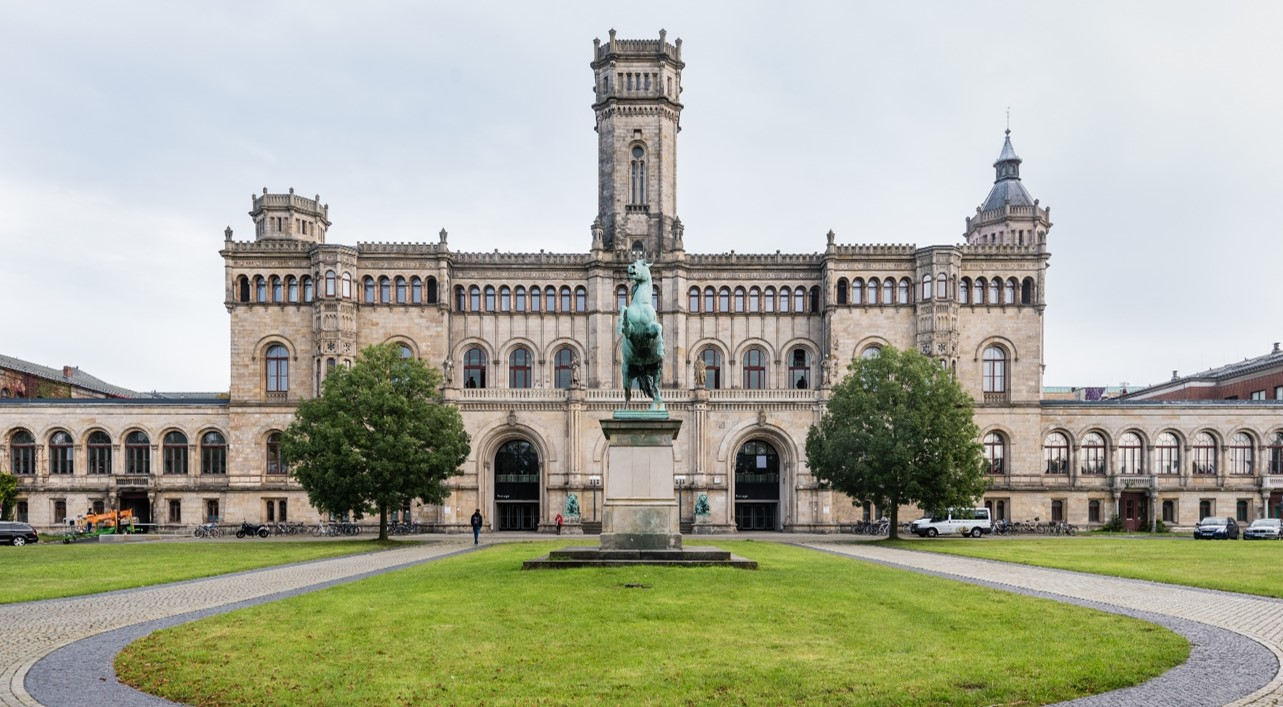
\includegraphics[width=0.65\textwidth]{figures/luh_default_presentation_title_image.jpg}}

% Title page: luhstyle
% \setbeamertemplate{title page}[luhstyle]
% % Add optional title image here
% \addtitlepageimage{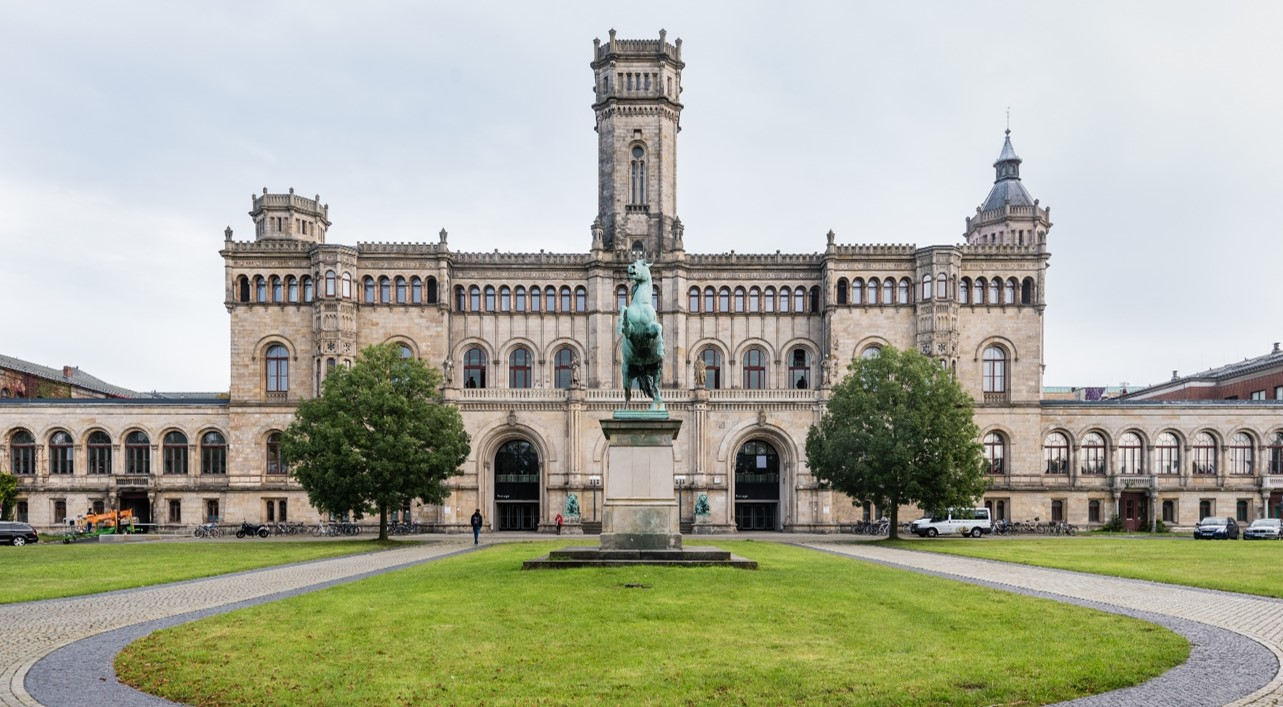
\includegraphics[width=0.75\textwidth]{figures/luh_default_presentation_title_image.jpg}}

\author[Abedjan \& Lindauer]{Ziawasch Abedjan \& Marius Lindauer\\[1em]
	
\includegraphics[height=\logoheight]{../latex_main/figures/luh_logo_rgb_0_80_155.pdf}\qquad
	
\includegraphics[height=\logoheight]{../latex_main/figures/DBIS_Kurzlogo.png}\qquad

\includegraphics[height=\logoheight]{../latex_main/figures/TNT_darkv4}\qquad

\includegraphics[height=\logoheight]{../latex_main/figures/L3S.jpg}	}
\date{Summer Term 2022; \hspace{0.5em} {
\includegraphics[height=1.5em]{../latex_main/figures/Cc-by-nc-sa_icon.svg.png}}; based on \href{https://ds100.org/fa21/}{[DS100]}
}


%%% Custom Packages
%----------------------------------------------------------------------
% Create dummy content
\usepackage{blindtext}

% Adds a frame with the current page layout. Just call \layout inside of a frame.
\usepackage{layout}


%%% Macros
%\renewcommand{\vec}[1]{\mathbf{#1}}
% \usepackage{bm}
%\let\vecb\bm

\title[Introduction]{DS: Pandas, Part 2}
\subtitle{Advanced Pandas syntax, aggregation, and joining}

\graphicspath{ {./figure/} }
%\institute{}


\begin{document}
	
	\maketitle
	
	\begin{frame}[c]{Announcements}
	    Quick note: In this class, I use the terms “method” and “function” interchangeably. 
	    
	    For example:
	    \begin{itemize}
	        \item df.value\_counts() is a method. It is also a function.

	    \end{itemize}

	\end{frame}
	
	\begin{frame}[c]{New Syntax / Concept Summary}
	    \begin{itemize}
	        \item Operations on String series, e.g. babynames[“Name”].str.startswith()
	        \item Creating and dropping columns.
	        \begin{itemize}
	            \item Creating temporary columns is often convenient for sorting.
	        \end{itemize}
	        \item Passing an index as an argument to loc.
	        \begin{itemize}
	            \item Useful as an alternate way to sort a dataframe.
	        \end{itemize}
            \item Groupby: Output of .groupby(“Name”) is a DataFrameGroupBy object. Condense back into a DataFrame or Series with:
            \begin{itemize}
                \item groupby.agg
                \item groupby.size
                \item groupby.filter
                \item and more...
            \end{itemize}
            \item Pivot tables: An alternate way to group by exactly two columns.
            \item Merge: A method to join two dataframes
	    \end{itemize}

	\end{frame}
	
	
	\begin{frame}[c]{Structure For Today}
	    Today we’ll introduce additional syntax by trying to solve various practical problems on our baby names dataset.

	    \begin{itemize}
	        \item Goal 1: Find the most popular name in California in 2018 (done in lec 4).
	        \item Goal 2: Find all names that start with J.
	        \item Goal 3: Sort names by length.
            \item Goal 4: Find the name whose popularity has changed the most.
            \item Goal 5: Count the number of female and male babies born in each year.
	    \end{itemize}
    
        We will also play around with our election dataset.\\
        You’ll get a chance to practice this syntax in next week’s lab and homework.

	\end{frame}
	
	
	
	\begin{frame}[c]{Str}

	\end{frame}
	
	
	\begin{frame}[c]{Manipulating String Data}
	    Goal 1: Find all rows where the Name starts with J.
	    
        One way using just the Python you learned in 61A / CS 88 would be to use a list comprehension to build a boolean array.
        
	\end{frame}
	
	
	\begin{frame}[c]{Manipulating String Data}
	    Suppose we want to find all rows where the Name starts with J.\\
	    Approach 1: Use list comprehensions from 61A/CS88.
	    \begin{itemize}
	        \item Create a list of booleans where ith entry is True if ith name starts with J.
	        \item Pass this list to [] or loc[].
	    \end{itemize}
        \hfill
        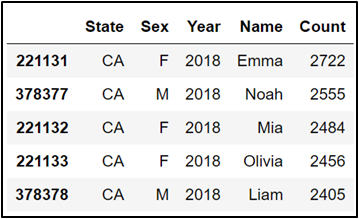
\includegraphics[scale=.75]{Bild1}
	\end{frame}
	
	
	
	\begin{frame}[c]{Manipulating String Data}
	    Suppose we want to find all rows where the Name starts with J.\\
	    Approach 1: Use list comprehensions from 61A/CS88.
	    \begin{itemize}
	        \item Create a list of booleans where ith entry is True if ith name starts with J.
	        \item Pass this list to [] or loc[].
	    \end{itemize}
        Goal: Fill the list comprehension ??? so that it returns the desired list.
        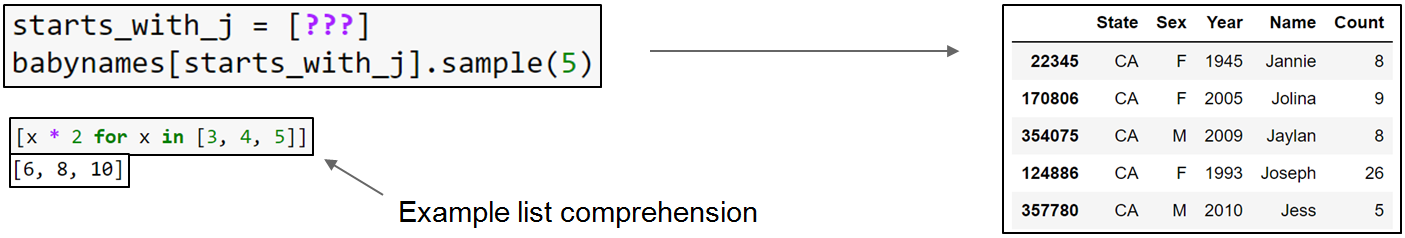
\includegraphics[scale=.4]{Bild2}
	\end{frame}
	
	
	\begin{frame}[c]{Manipulating String Data}
	    Suppose we want to find all rows where the Name starts with J.\\
	    Approach 1: Use list comprehensions from 61A/CS88.
	    \begin{itemize}
	        \item Create a list of booleans where ith entry is True if ith name starts with J.
	        \item Pass this list to [] or loc[].
	    \end{itemize}
        Goal: Write a list comprehension that returns the desired list.
        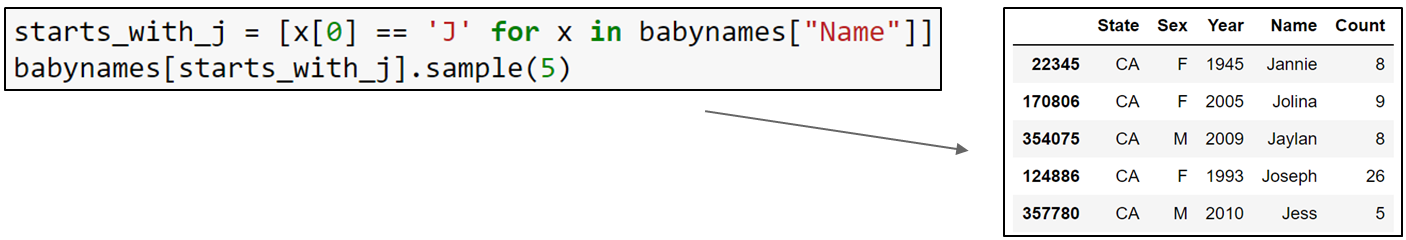
\includegraphics[scale=.4]{Bild3}
	\end{frame}
	
	
	\begin{frame}[c]{A More Advanced Approach}
	    Approach 1: Use a list comprehensions.\\
	    \hspace{1cm}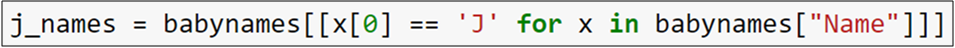
\includegraphics[scale=.5]{Bild4}\\
	    Approach 2: Use a str method from the Series class (more on this shortly).\\
	    \hspace{1cm}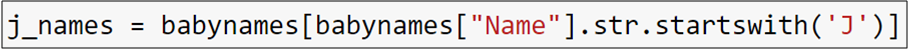
\includegraphics[scale=.5]{Bild5}\\
        Question: What’s better about this second approach?
        \begin{itemize}
            \item More readable! Others can understand your code. ← the main great thing
            \item First one is likely to be less efficient.
        \end{itemize}
	\end{frame}
	
	
	\begin{frame}[c]{Idiomatic Code}
	    Approach 1: Use a list comprehensions.\\
	    \hspace{1cm}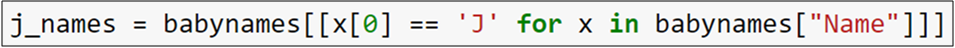
\includegraphics[scale=.5]{Bild4}\\
	    Approach 2: Use a str method from the Series class (more on this shortly).\\
	    \hspace{1cm}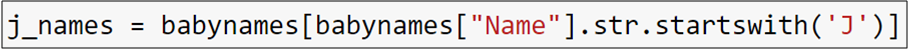
\includegraphics[scale=.5]{Bild5}\\
        Terminology note: We say that approach #1 is not idiomatic.

        \begin{itemize}
            \item Idiom: “the language peculiar to a people or to a district, community, or class.”
            \item In other words, people from the broader pandas community won’t like reading your code if it looks like approach 1.
        \end{itemize}
	\end{frame}
	
	
	\begin{frame}[c]{Str Methods}
	    The str methods from the Series class have pretty intuitive behavior.
	    \begin{itemize}
	        \item Won’t define formally. Full list at bottom of [this link].
	    \end{itemize}
	    Example: str.startswith
	    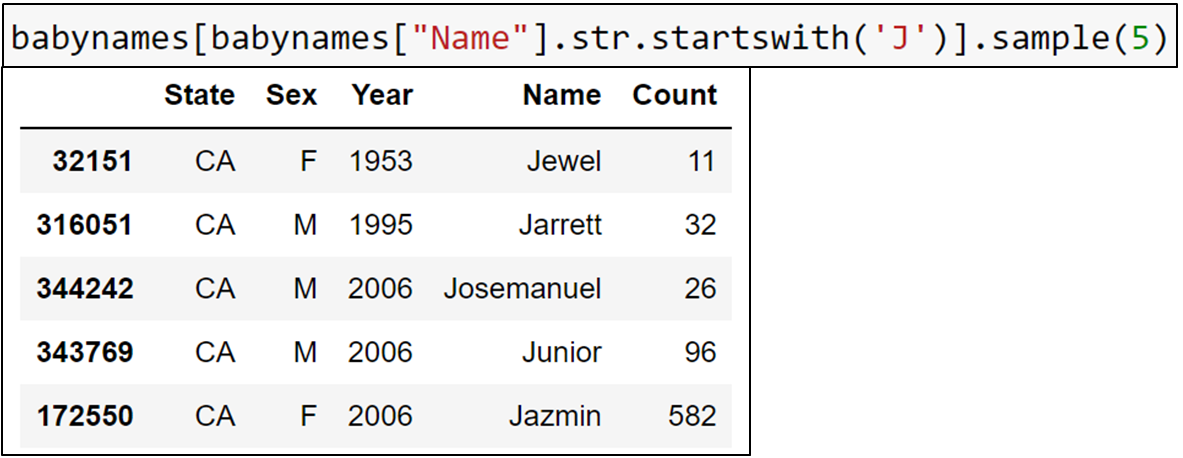
\includegraphics[scale=.44]{Bild6}\\
	\end{frame}
	
	
	
	\begin{frame}[c]{Str Methods}
	    The str methods from the Series class have pretty intuitive behavior.
	    \begin{itemize}
	        \item Won’t define formally. Full list at bottom of [this link].
	    \end{itemize}
	    Example: str.contains
	    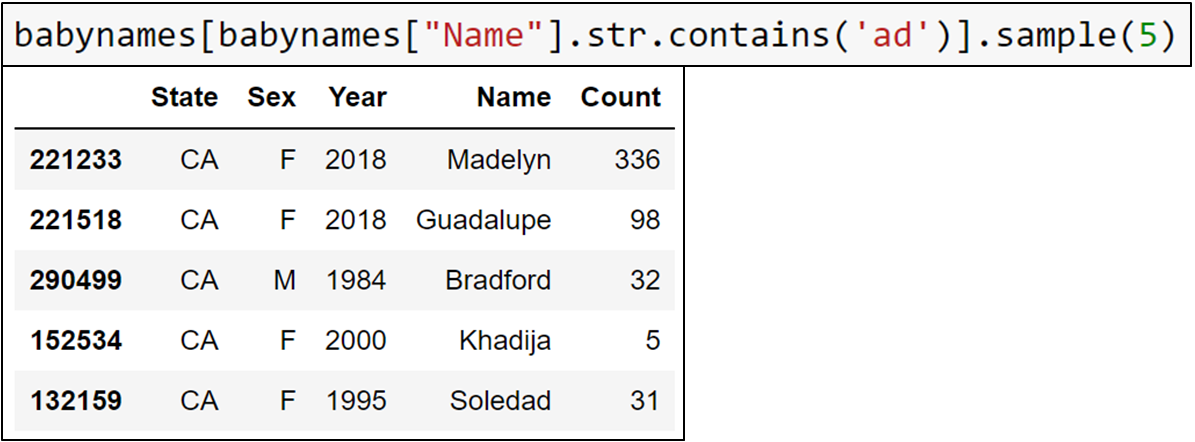
\includegraphics[scale=.44]{Bild7}\\
	\end{frame}
	
	
	
	\begin{frame}[c]{Str Methods}
	    The str methods from the Series class have pretty intuitive behavior.
	    \begin{itemize}
	        \item Won’t define formally. Full list at bottom of [this link].
	    \end{itemize}
	    Example: str.split
	    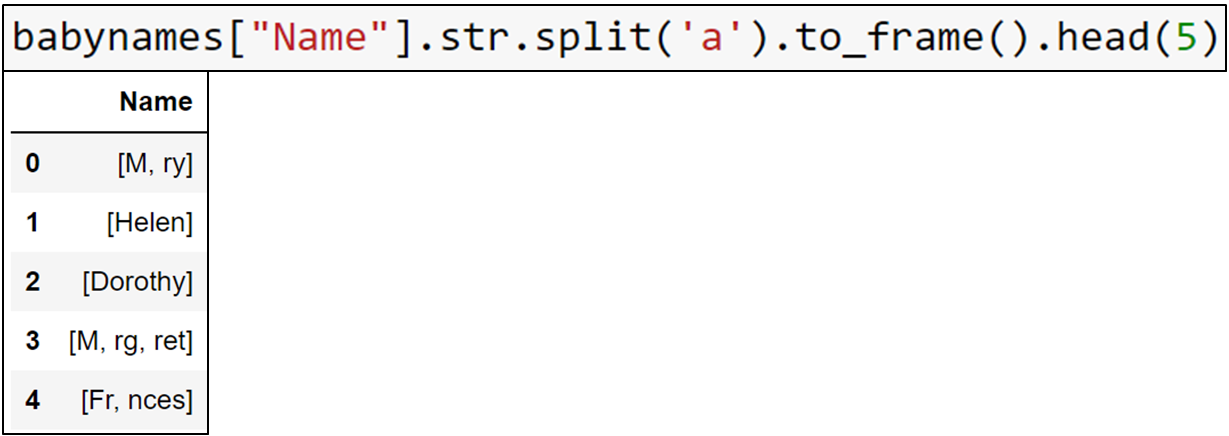
\includegraphics[scale=.44]{Bild8}\\
	\end{frame}
	
	
	
	\begin{frame}[c]{Challenge}
	    Write a line of code that creates a list (or Series or array) of all names that end with “ert”.
	    \begin{itemize}
	        \item Your list should have only one instance of each name!
	    \end{itemize}
	    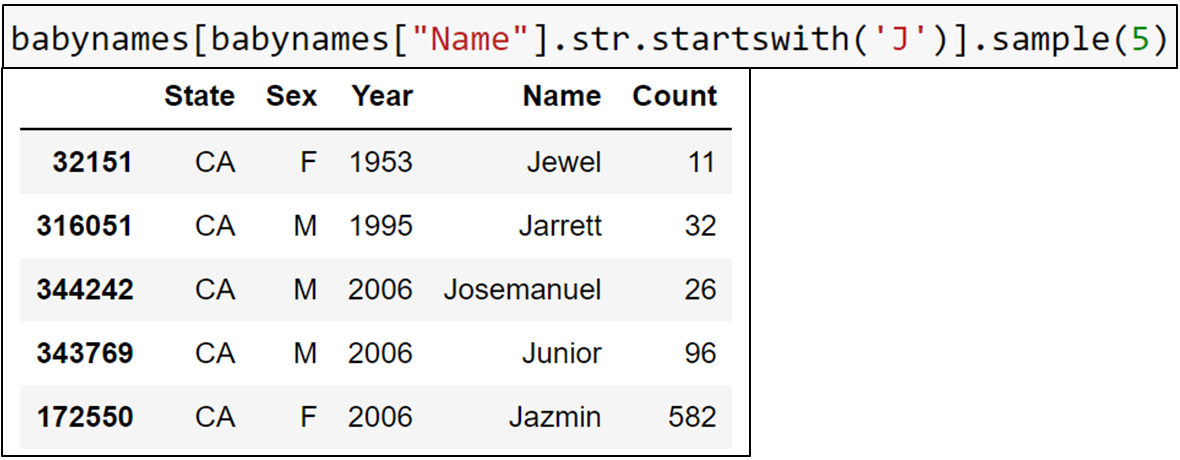
\includegraphics[scale=.44]{Bild9}\\
	\end{frame}
	
	
	\begin{frame}[c]{Challenge}
	    Write a line of code that creates a list (or Series or array) of all names that end with “ert”.
	    \begin{itemize}
	        \item Your list should have only one instance of each name!
	    \end{itemize}
	    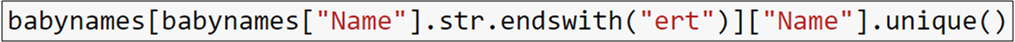
\includegraphics[scale=.74]{Bild10}\\
	\end{frame}
	
	\begin{frame}{Adding, Modifying, and Removing Columns}
	    
	\end{frame}
	
	
	\begin{frame}[c]{Sorting By Length}
	   Goal 3: Sort our baby names by length. \\
	   \bigskip
	   The sort\_values function does not provide the ability to pass a custom comparison function.\\
	   \bigskip
	   Lots of weird ways to do this, e.g. from last year’s Spring 19 lecture:\\
	   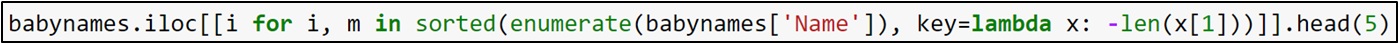
\includegraphics[scale=.65]{Bild11}\\
	    Let’s see two different ways of doing this that are much nicer.
	    \begin{itemize}
	        \item Approach 1: Creating a temporary column, then sort on it.
	        \item Approach 2: Creating a sorted index and using loc.
	    \end{itemize}
	    
	\end{frame}
	
	
	\begin{frame}[c]{Approach 1: Create a Temporary Column}
        Intuition: Create a column equal to the length. Sort by that column.

	   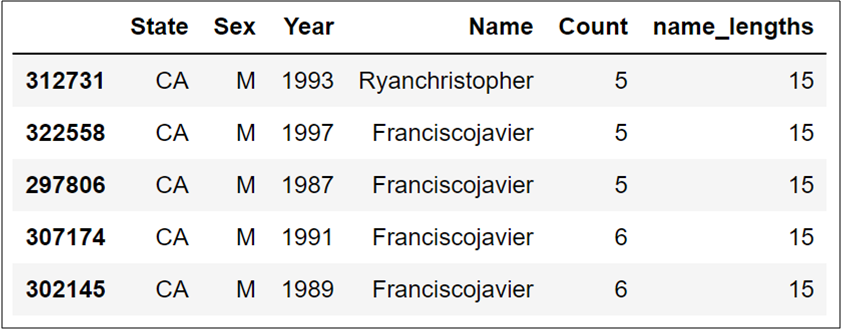
\includegraphics[scale=.74]{Bild12}\\
	\end{frame}
	
	
	\begin{frame}[c]{Syntax for Column Addition}
        Adding a column is easy:

    \hfill
	   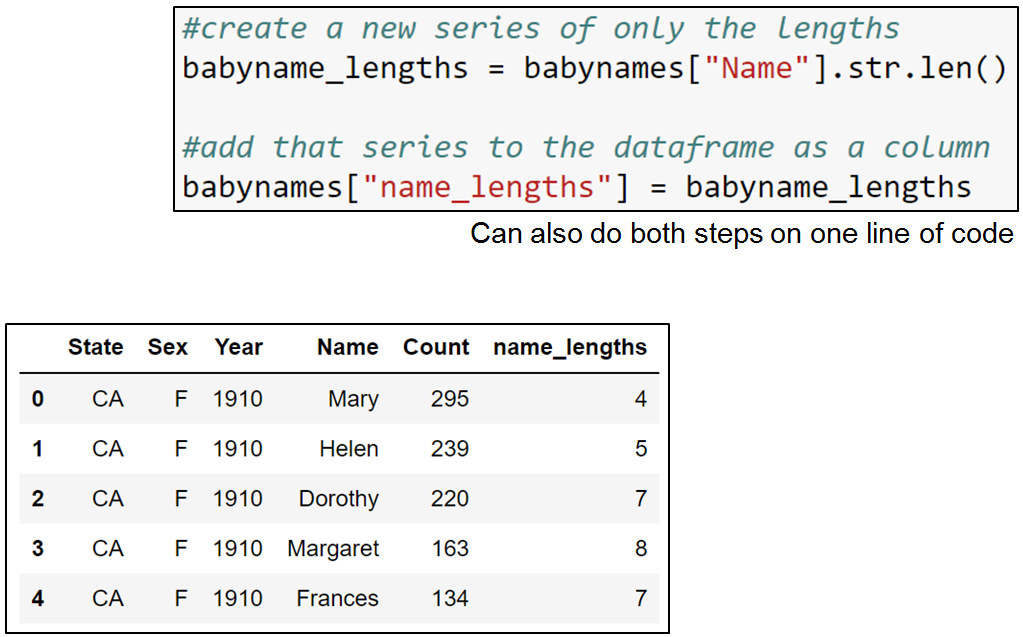
\includegraphics[scale=.37]{Bild13}\\
	\end{frame}
	
	
	\begin{frame}[c]{Syntax for Dropping a Column (or Row)}
        After sorting, we can drop the temporary column.
        \begin{itemize}
            \item The Drop method assumes you’re dropping a row by default. Use axis = 1 to drop a column instead.
        \end{itemize}
	   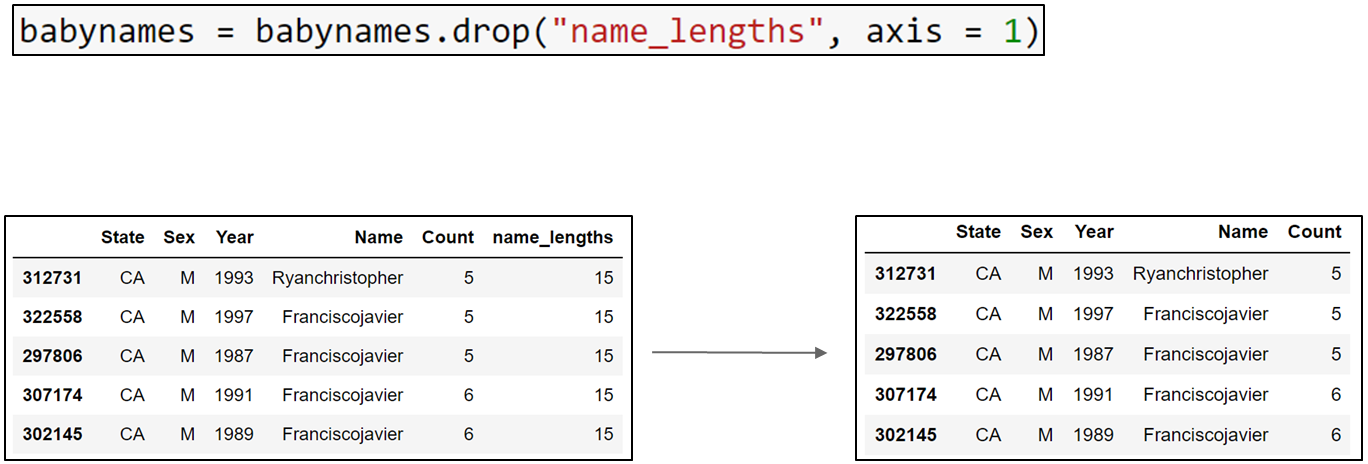
\includegraphics[scale=.37]{Bild14}\\
	\end{frame}
	
	
	\begin{frame}[c]{Sorting by Arbitrary Functions}
       Suppose we want to sort by the number of occurrences of “dr” + number of occurrences of “ea”.
        \begin{itemize}
            \item Use the Series .map method.
        \end{itemize}
	   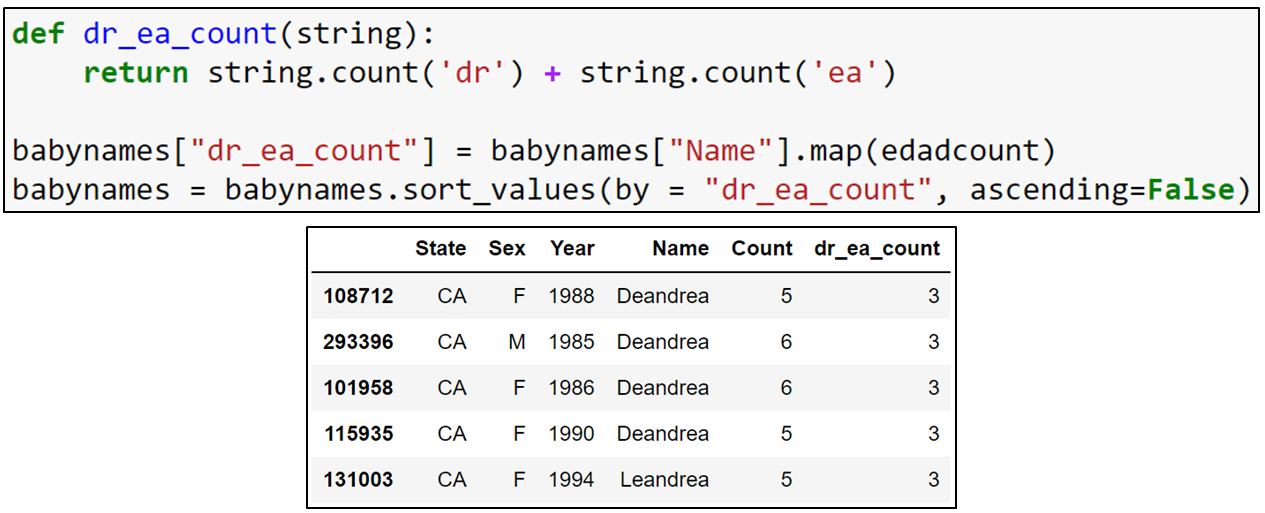
\includegraphics[scale=.37]{Bild15}\\
	\end{frame}
	
	
	\begin{frame}{A Little More .loc}
	    
	\end{frame}
	
	
	
	\begin{frame}[c]{Sorting By Length}
        Goal 3: Sort our baby names by length. \\
        The sort\_values function does not provide the ability to pass a custom comparison function.\\
        Let’s see two different ways of doing this that are much nicer.

        \begin{itemize}
            \item Approach 1: Creating a temporary column, then sort on it.
            \item Approach 2: Creating a sorted index and using loc.
        \end{itemize}
	\end{frame}
	
	
	\begin{frame}[c]{Approach 2: Create a Sorted Index and Pass to .loc}
        Another approach is to take advantage of another feature of .loc.

        \begin{itemize}
            \item df.loc[idx] returns the DataFrame in the same order as the given index.
            \item Only works if the index exactly matches the DataFrame.

        \end{itemize}
        Let’s see this approach in action.
	\end{frame}
	
	
	\begin{frame}[c]{Approach 2: Create a Sorted Index and Pass to .loc}
       Step 1: Create Series of only the lengths of the names.
        \begin{itemize}
            \item This Series will have the same index as the original DataFrame.
        \end{itemize}
	   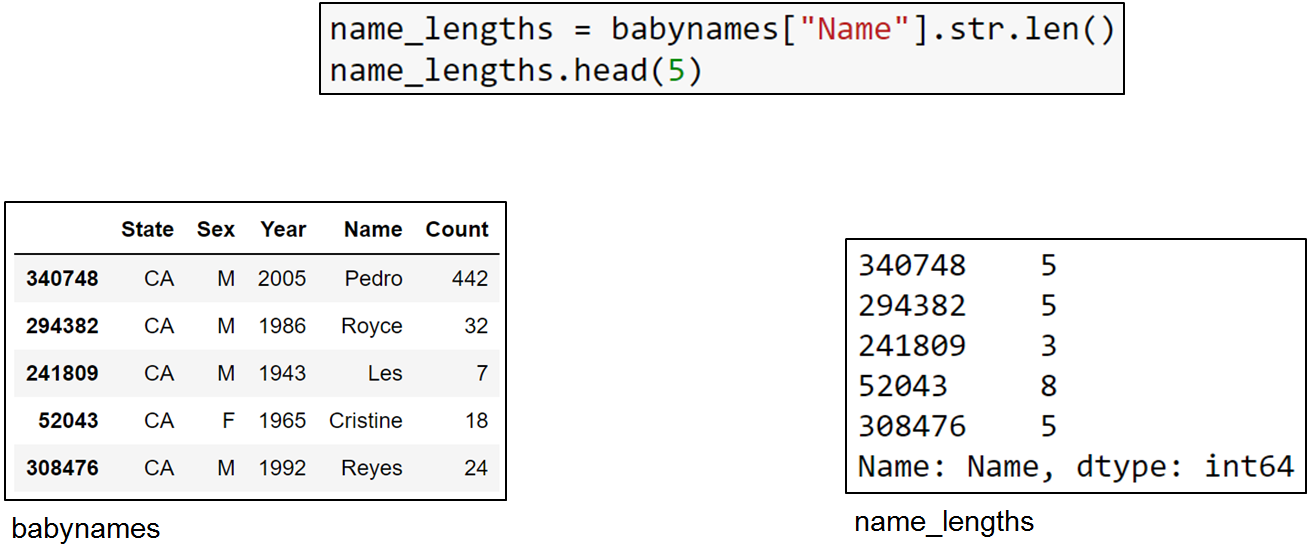
\includegraphics[scale=.37]{Bild16}\\
	\end{frame}
	
	
	
	
	\begin{frame}[c]{Approach 2: Create a Sorted Index and Pass to .loc}
       Step 2: Sort the series of only name lengths.
        \begin{itemize}
            \item This Series will have an index which is reordered relative to the original dataframe.
        \end{itemize}
	   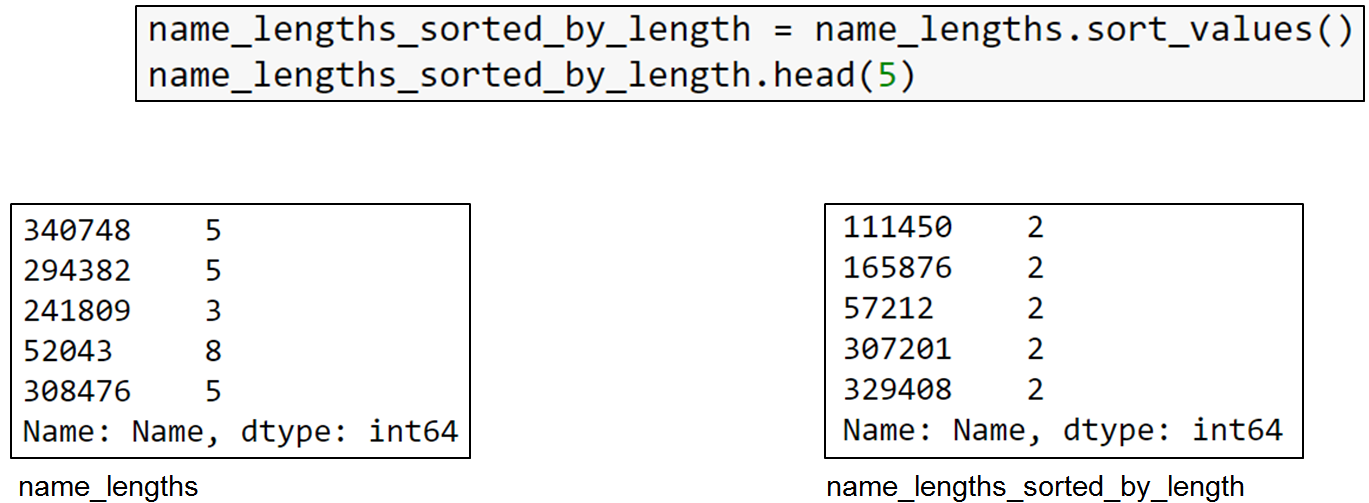
\includegraphics[scale=.37]{Bild17}\\
	\end{frame}
	
	
    \begin{frame}[c]{Approach 2: Create a Sorted Index and Pass to .loc}
       Step 3: Pass the sorted index as an argument of .loc to the original dataframe.

	   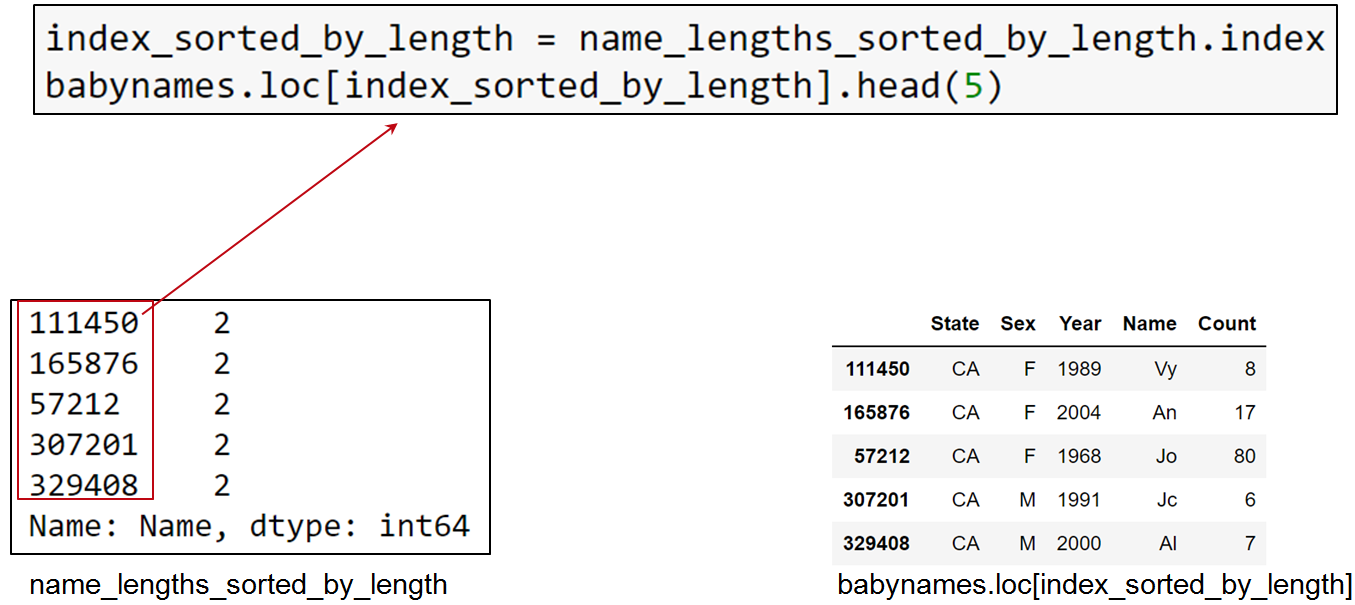
\includegraphics[scale=.37]{Bild18}\\
	\end{frame}


    \begin{frame}{groupby.agg}
        
    \end{frame}
    
    
    \begin{frame}{Sorting By Length}
        Goal 4: Find the names that have changed the most in popularity.\\
        \bigskip
        Let’s start by defining what we mean by changed popularity.
        \begin{itemize}
            \item In lecture, let’s stay simple and use the AMMD (absolute max/min difference): max(count) - min(count). %Note: This is not a common term. I just made it up.


        \end{itemize}
        \bigskip
        Example for “Jennifer”:
        \begin{itemize}
            \item In 1954, there were only 5.
            \item In 1972, we hit peak Jennifer. 6,066 Jennifers were born.
            \item AMMD is 6,066 - 5 = 6,061.
        \end{itemize}
    \end{frame}
    
    
    
    \begin{frame}{Sorting By Length}
        Goal 4: Find the names that have changed the most in popularity.\\
        \bigskip
        Let’s start by defining what we mean by changed popularity.
        \begin{itemize}
            \item In lecture, let’s stay simple and use the AMMD (absolute max/min difference): max(count) - min(count). %Note: This is not a common term. I just made it up.


        \end{itemize}
        \bigskip
        Example for “Jennifer”:
        \begin{itemize}
            \item In 1954, there were only 5.
            \item In 1972, we hit peak Jennifer. 6,066 Jennifers were born.
            \item AMMD is 6,066 - 5 = 6,061.
        \end{itemize}
    \end{frame}
    
    
    
    \begin{frame}{Example: Computing the AMMD for a Given Name}
        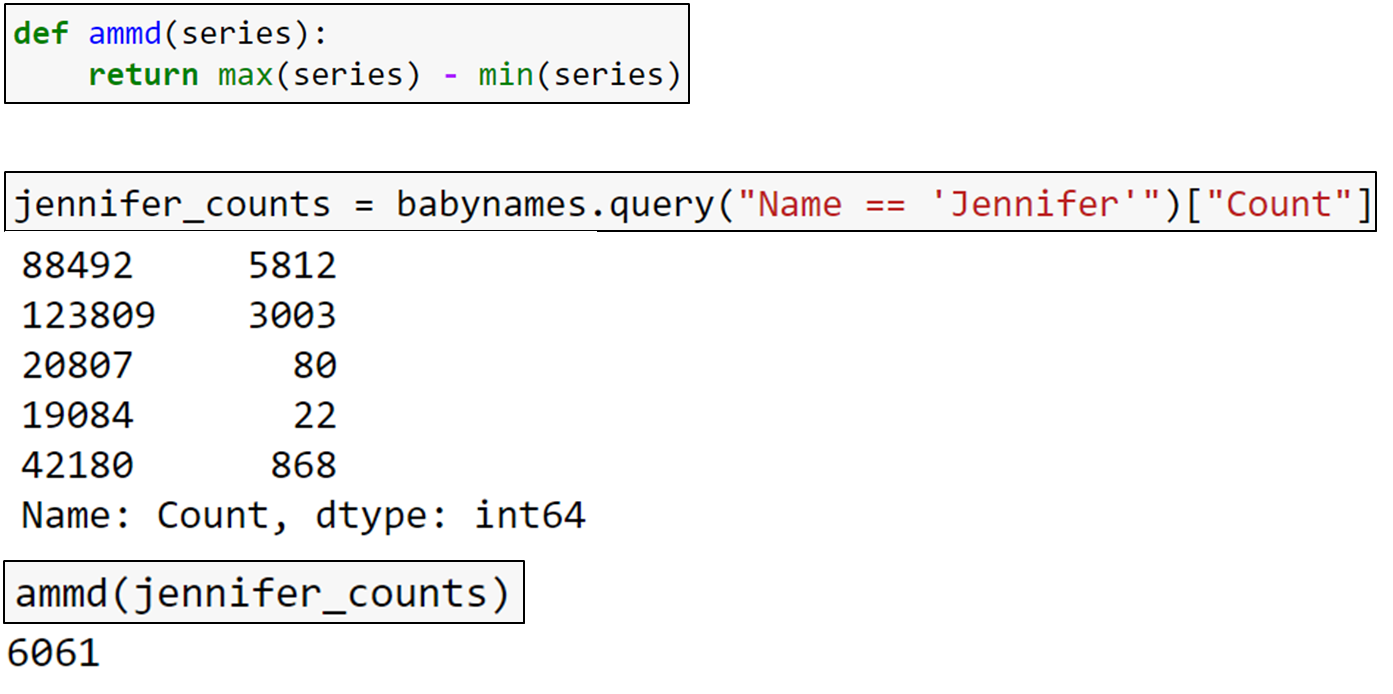
\includegraphics[scale=.4]{Bild19}
    \end{frame}
    
    
    \begin{frame}{Approach 1: Getting AMMD for Every Name The Hard Way}
    Approach 1: Hack something together using our existing Python knowledge.
        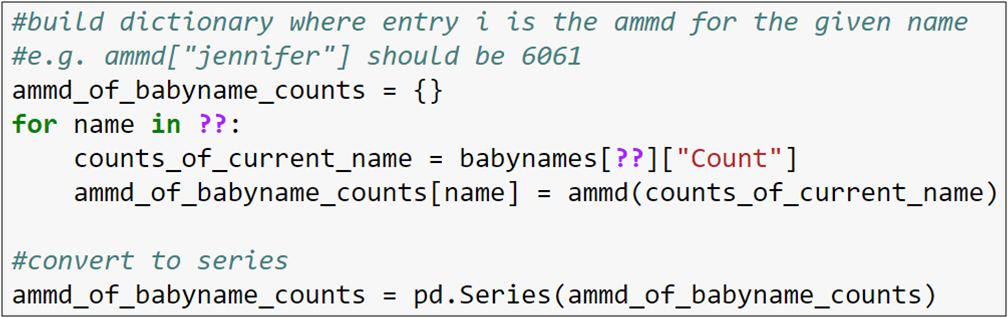
\includegraphics[scale=.67]{Bild20}
        
    Challenge: Try to fill in the code above.

    \end{frame}
    
    
    
    \begin{frame}{Approach 1: Getting AMMD for Every Name The Hard Way}
    Approach 1: Hack something together using our existing Python knowledge.
        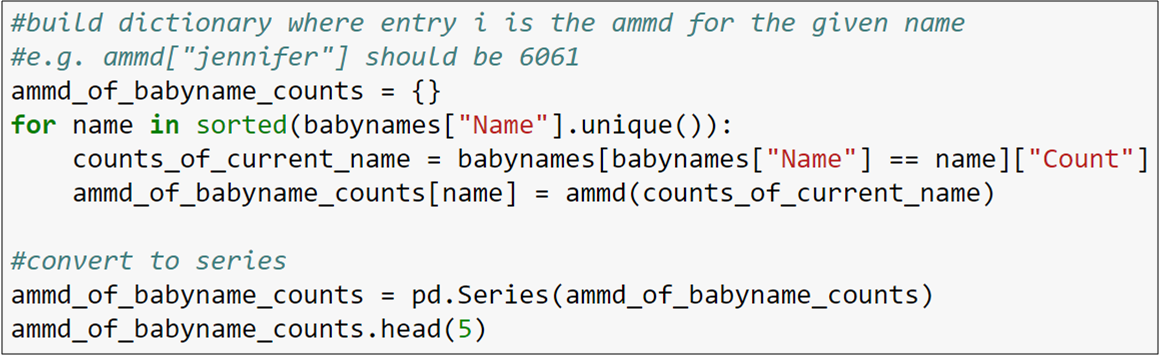
\includegraphics[scale=.64]{Bild21}
        
    The code above is extremely slow, and also way more complicated than the better approach coming next.


    \end{frame}
    
    
    \begin{frame}{Approach 2: Using Groupby and Agg}
        The code below is the more idiomatic way of computing what we want.
        \begin{itemize}
            \item Much simpler, much faster, much more versatile.
        \end{itemize}
        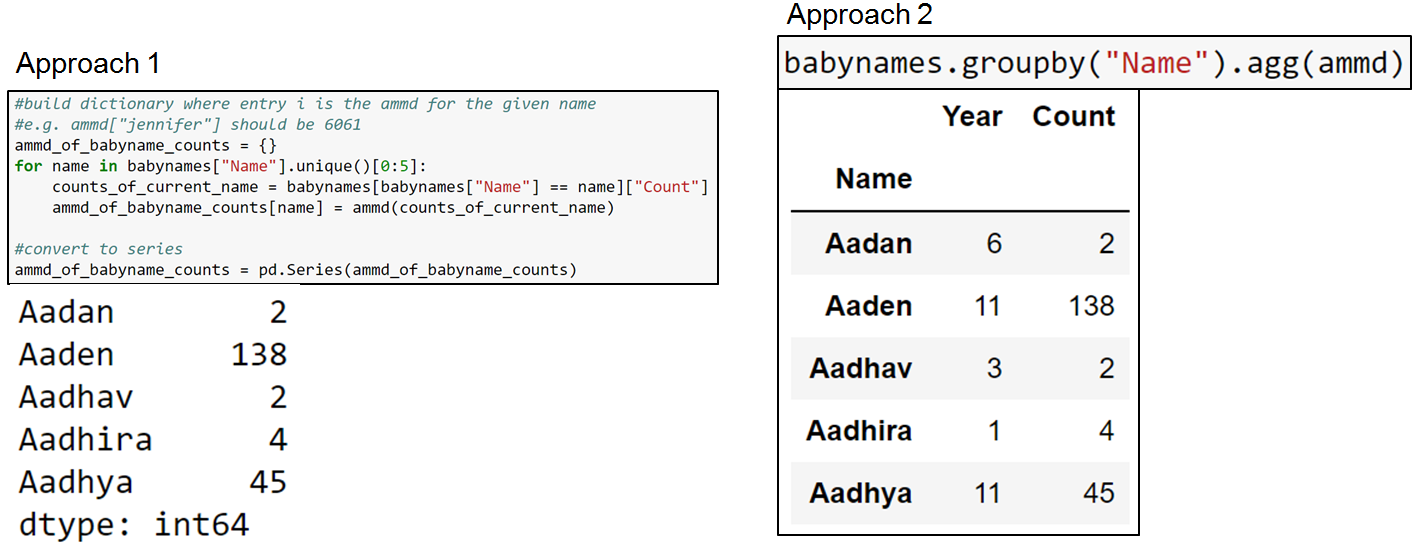
\includegraphics[scale=.39]{Bild22}
    \end{frame}
    
    
    
    \begin{frame}{Attendance Question: Check Your groupBy Understanding}
        Approach 2 generated two columns, Year and Count. yellkey.com/stella
        
        \begin{columns}
            \begin{column}{.4\textwidth}
                    What do you think the Year column represents?
                    \begin{itemize}
                        \item[A]  The number of years a name appeared.
                        \item[B] The difference between the earliest and latest year a name appeared.
                        \item[C] It has no meaning because our code was only designed to work with counts.
                        \item[D] Not sure.
                    \end{itemize}
            \end{column}
            
            \begin{column}{.5\textwidth}
                    \begin{figure}
                        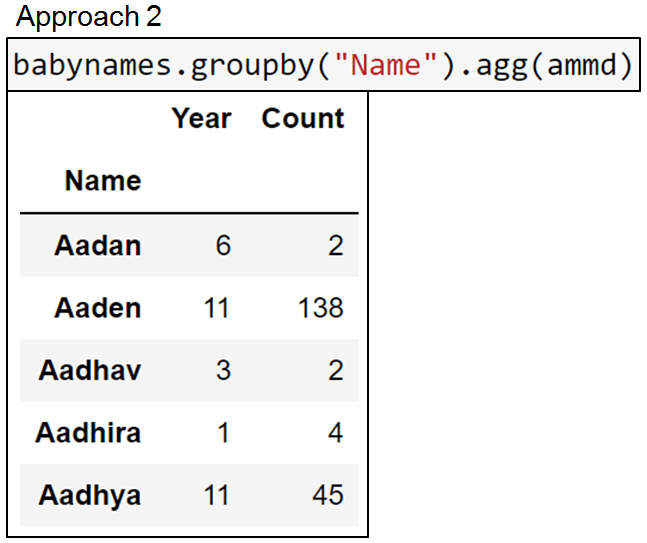
\includegraphics[scale=.37]{Bild23}
                    \end{figure}
            \end{column}
            
        \end{columns}
        
    \end{frame}
    
    
    
    
     \begin{frame}{Attendance Question: }
        Approach 2 generated two columns, Year and Count.
        
        \begin{columns}
            \begin{column}{.4\textwidth}
                    What do you think the Year column represents?
                    \begin{itemize}
                        \item[A]  The number of years a name appeared.
                        \item[B] \textbf{The difference between the earliest and latest year a name appeared.}
                        \item[C] It has no meaning because our code was only designed to work with counts.
                        \item[D] Not sure.
                    \end{itemize}
            \end{column}
            
            \begin{column}{.5\textwidth}
                    \begin{figure}
                        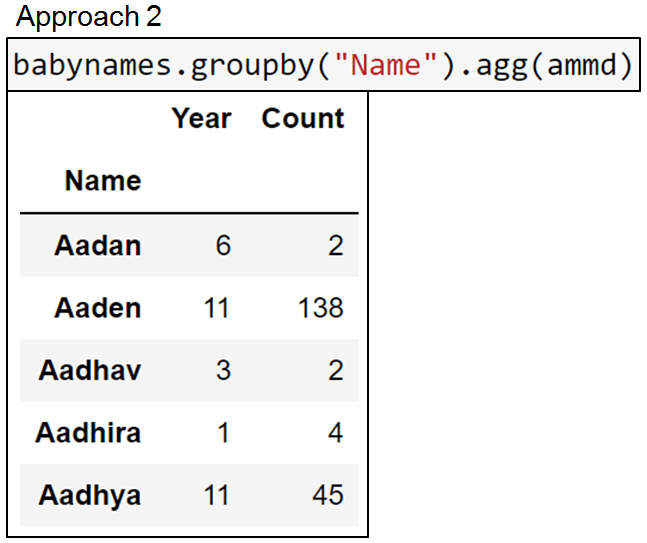
\includegraphics[scale=.37]{Bild23}
                    \end{figure}
            \end{column}
            
        \end{columns}
        
    \end{frame}
    
    
    
    \begin{frame}{DataFrame groupby.agg Visually}
        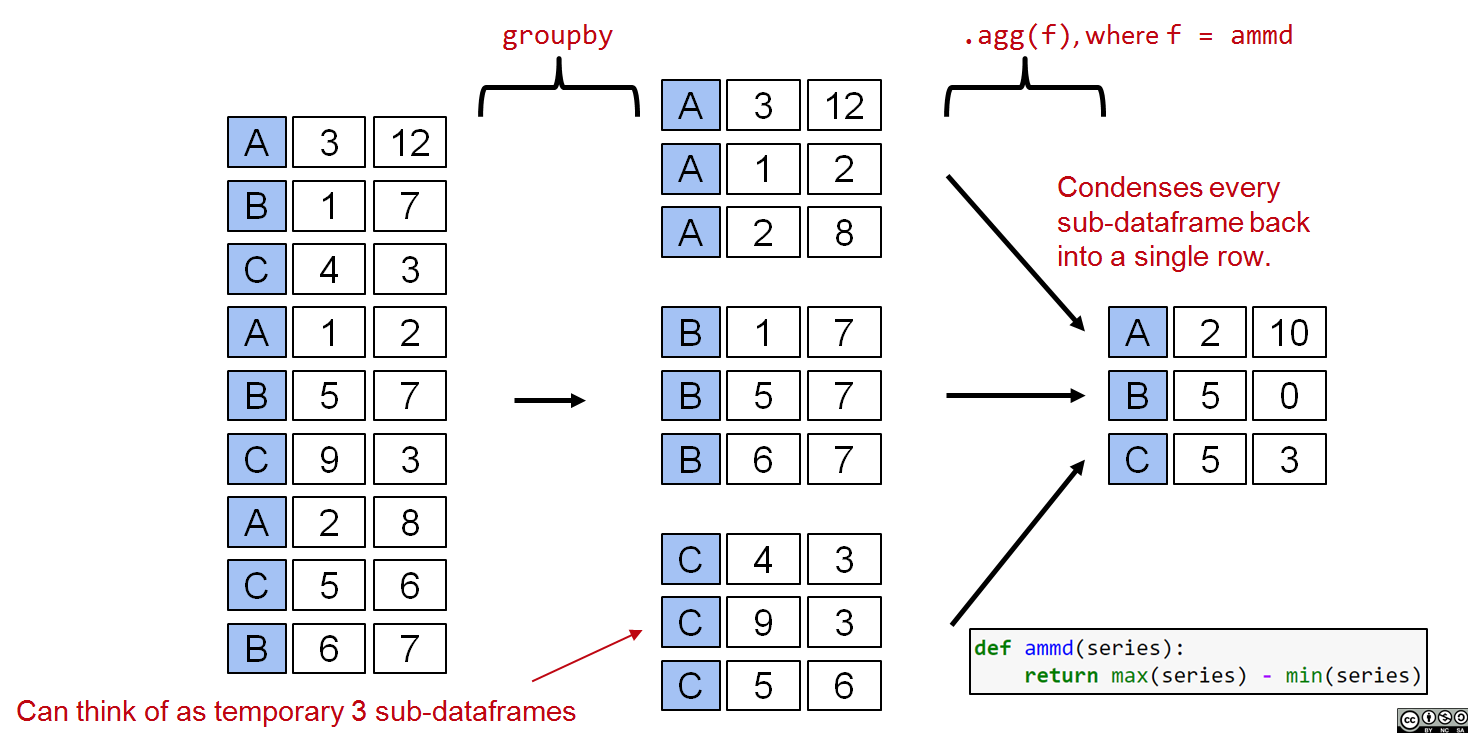
\includegraphics[scale=.34]{Bild24}
    \end{frame}
    
    
    \begin{frame}{Some groupby.agg puzzles}
        
    \end{frame}
    
    
    
    \begin{frame}{groupby Puzzle \#1}
    Below, we show the result of the given code. What does it mean?
        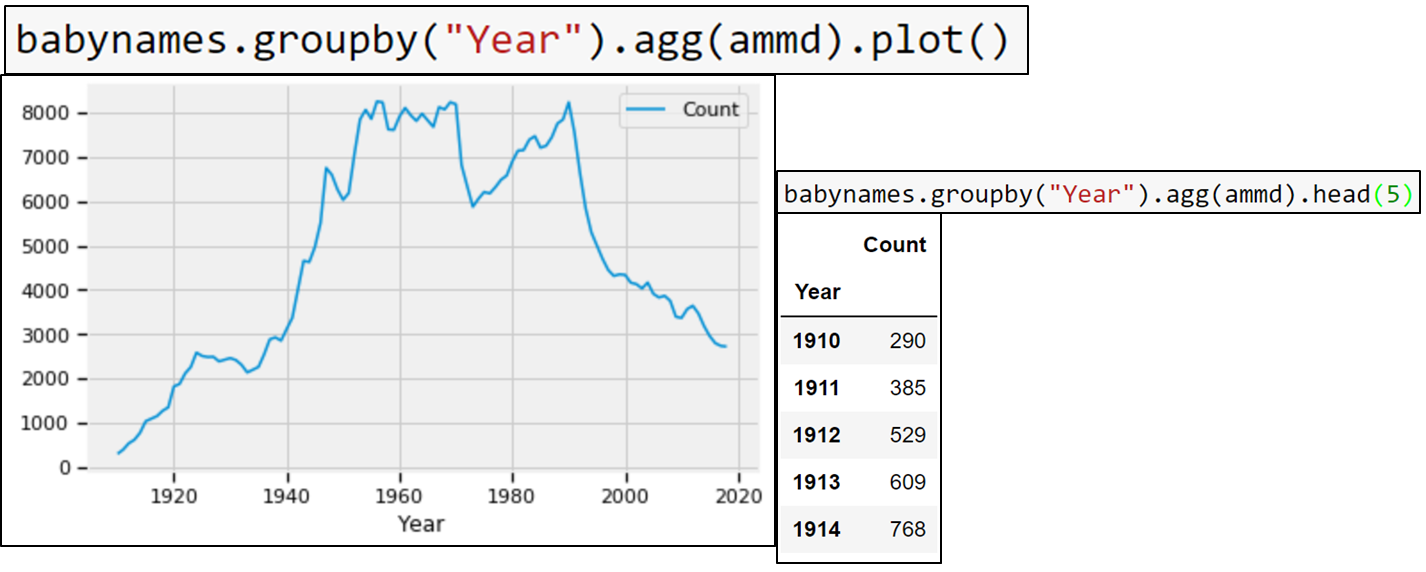
\includegraphics[scale=.4]{Bild25}
    \end{frame}
    
    
    
    \begin{frame}{groupby Puzzle \#2}
    Be careful when using groupby. Consider the results on our elections table:
        \centering
        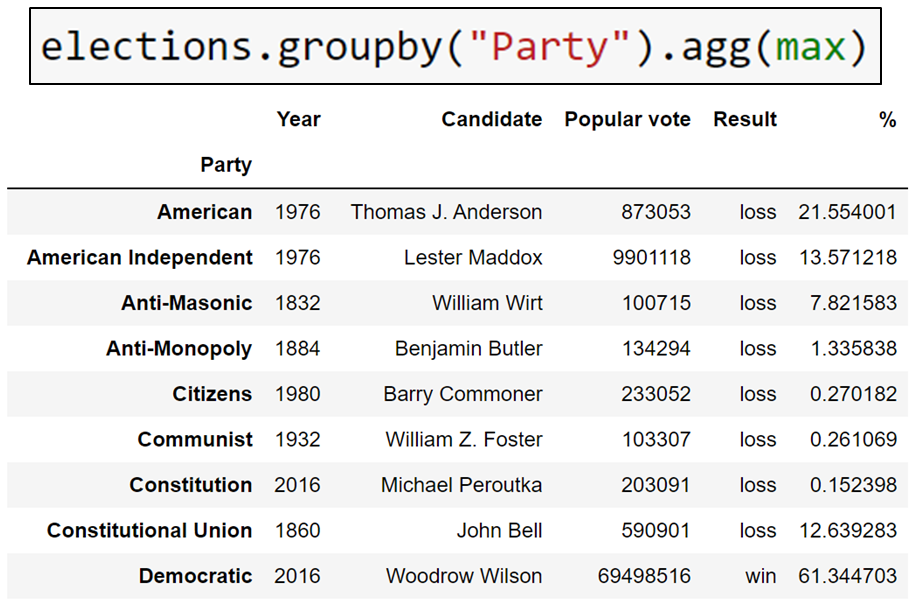
\includegraphics[scale=.38]{Bild26}
    \end{frame}
    
    
    \begin{frame}{groupby Puzzle \#2}
    Why does the table seem to claim that Woodrow Wilson won the presidency in 2016?

        \centering
        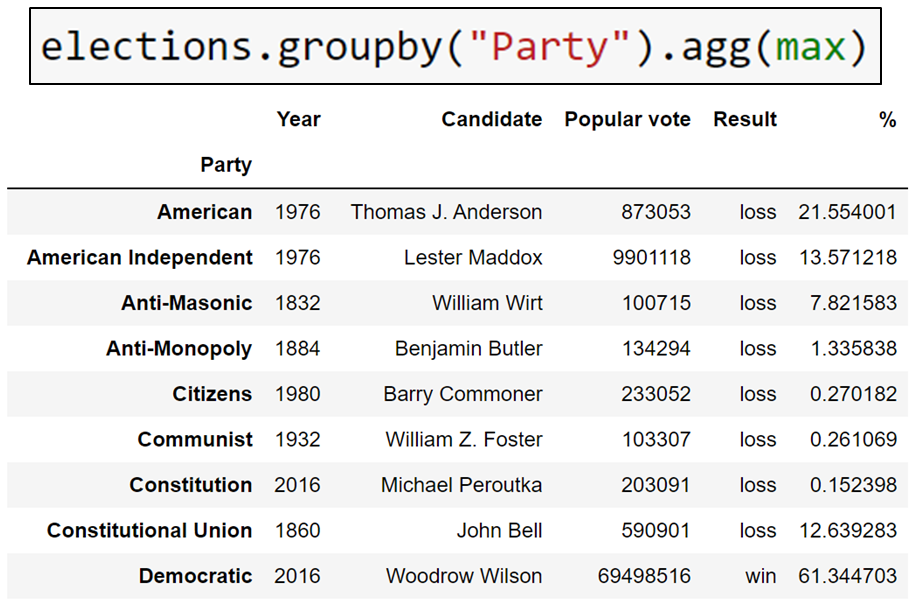
\includegraphics[scale=.38]{Bild26}
    \end{frame}
    
    
    
    \begin{frame}{groupby Puzzle \#2}
    Why does the table seem to claim that Woodrow Wilson won the presidency in 2016?
    \begin{columns}
        
    \begin{column}{.4\textwidth}
            Every column is calculated independently! Among Democrats:
            \begin{itemize}
                \item Last year they ran: 2016
                \item Alphabetically latest candidate name: Woodrow Wilson
                \item Highest \% of vote: 61.34
            \end{itemize}
    \end{column}
    \begin{column}{.5\textwidth}
        \begin{figure}
             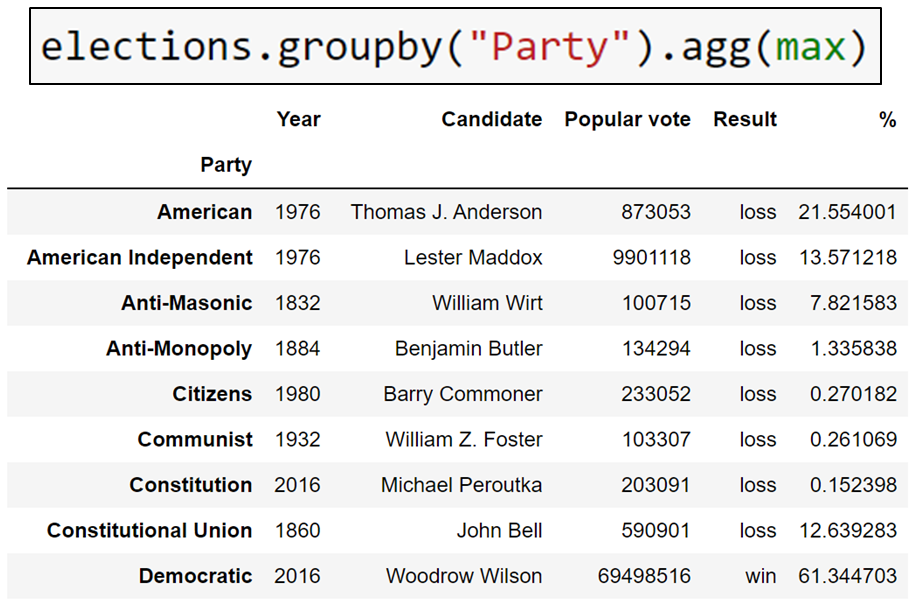
\includegraphics[scale=.28]{Bild26}
        \end{figure}
    \end{column}
       
        
    \end{columns}
    \end{frame}
    
    
    
     \begin{frame}{groupby Puzzle \#3}

        \centering
        
\includegraphics[scale=.36]{Bild28}
    \end{frame}
    
    \begin{frame}{groupby Puzzle \#3}

        \centering
        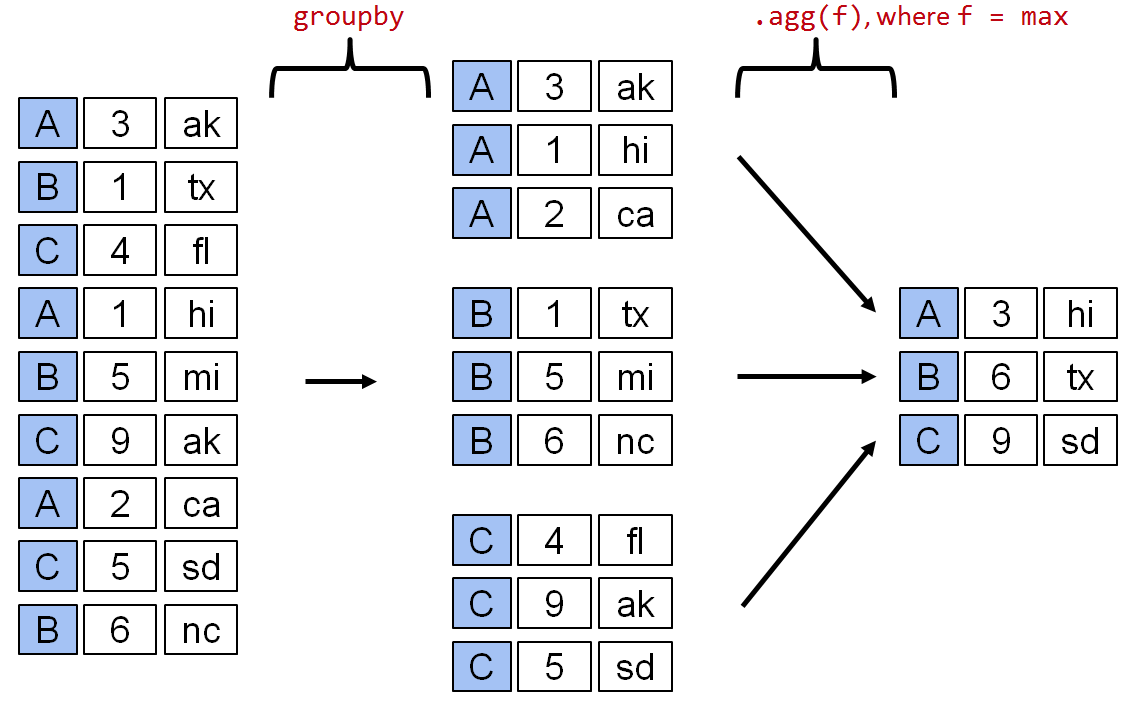
\includegraphics[scale=.36]{Bild27}
    \end{frame}
    
    
     \begin{frame}{ Puzzle \#4}
        Very hard puzzle: Try to write code that returns the table below.
        \begin{itemize}
            \item Each row shows the best result (in \%) by each party.
            \begin{itemize}
                \item For example: Best Democratic result ever was Johnson’s 1964 win.
            \end{itemize}
        \end{itemize}
        \centering
        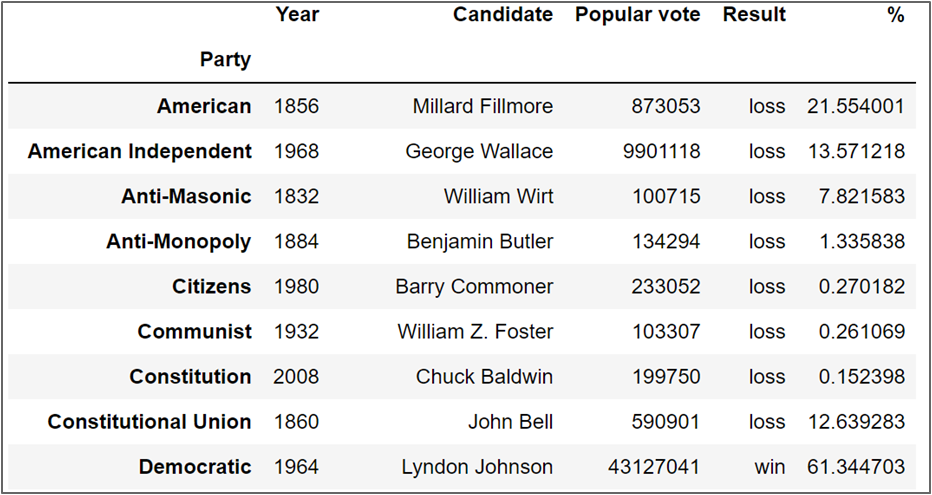
\includegraphics[scale=.56]{Bild29}
    \end{frame}
    
    
    
    \begin{frame}{ Puzzle \#4}
        Very hard puzzle: Try to write code that returns the table below.
        \begin{itemize}
            \item Hint, first do:  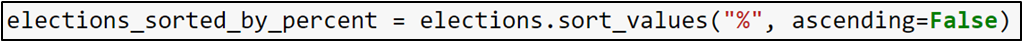
\includegraphics[scale=.7]{Bild30}
            \item Each row shows the best result (in \%) by each party.
        \end{itemize}
        \centering
        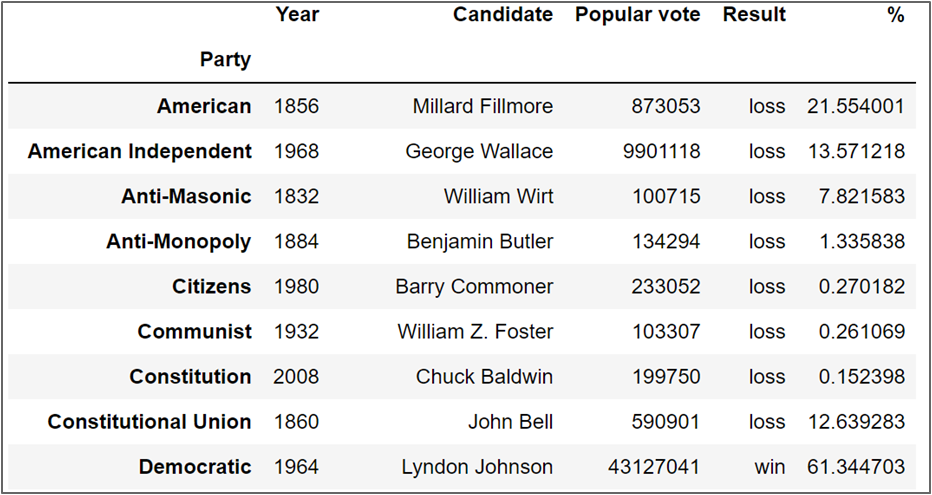
\includegraphics[scale=.56]{Bild29}
    \end{frame}
    
    
    
    \begin{frame}{ Puzzle \#4}
        Very hard puzzle: Try to write code that returns the table below.
        \begin{itemize}
            \item First sort the DataFrame so that rows are in ascending order of \%. 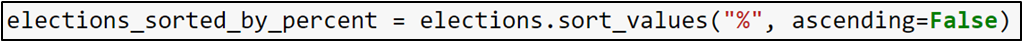
\includegraphics[scale=.7]{Bild30}
            \item Then group by Party and take the 0th member of each series. \includegraphics[scale=.7]{Bild31}

        \end{itemize}
        \hfill
        \includegraphics[scale=.45]{Bild29}
    \end{frame}
    
    
    
    \begin{frame}{Quick Note}
        If this type of programming seems scary, don’t worry, you’ll get used to it.
        \begin{itemize}
            \item Very different than the procedural style that you may be used to in Java, Matlab, Python, etc.
            \item Has a more declarative/SQL like feel.
        \end{itemize}
    \end{frame}
    
    
    \begin{frame}{Other groupby Features}
        
    \end{frame}
    
    
    
    \begin{frame}{Revisiting groupby.agg}
        So far, we’ve seen that df.groupby(“year”).agg(sum):
        \begin{itemize}
            \item Organizes all rows with the same year into a subframe for that year. 
            \item Creates a new dataframe with one row representing each subframe year.
            \begin{itemize}
                \item All rows in each subframe are combined using the sum function.
            \end{itemize}
        \end{itemize}
        \centering
        \includegraphics[scale=.38]{Bild32}
    \end{frame}
    
    
    
    \begin{frame}{Raw groupby Objects}
        The result of a groupby operation applied to a DataFrame is a DataFrameGroupBy object.
        \begin{itemize}
            \item It is not a DataFrame!
            \includegraphics[scale=.39]{Bild33}
        \end{itemize}
        Given a DataFrameGroupBy object, can use various functions to generate DataFrames (or Series). Agg is only one choice:
        \begin{itemize}
            \item agg: Creates a new DataFrame with one aggregated row per subframe.
            \item size: Creates a new Series with the size of each subframe.
            \item filter: Creates a copy of the original DataFrame, but keeping only rows from subframes that obey the provided condition.
        \end{itemize}
    \end{frame}
    
    
    
    \begin{frame}{groupby.size()}
        \centering
         \includegraphics[scale=.35]{Bild34}
    \end{frame}
    
    
    \begin{frame}{groupby.size()}
        Another common use for groups is to filter data.
        \begin{itemize}
            \item groupby.filter takes an argument f.
            \item f is a function that:
            \begin{itemize}
                \item Takes a DataFrame as input.
                \item Returns either true or false.
            \end{itemize}
            \item For each group g, f is applied to the subframe comprised of the rows from the original dataframe corresponding to that group.
        \end{itemize}
    \end{frame}
    
    
    
     \begin{frame}{groupby.filter}
       \centering
       \includegraphics[scale=.36]{Bild35}
    \end{frame}
    
    
    
    
    \begin{frame}{groupby.sum(), groupby.mean(), groupby.max(), etc...}
       For common operations, rather than saying e.g. groupby.agg(sum), we can instead do groupby.sum():\\
        \centering
       \includegraphics[scale=.36]{Bild36}
    \end{frame}
    
    
    
    
    \begin{frame}{groupby([]) and Pivot Tables}

    \end{frame}
    
    
    
    
    \begin{frame}{Grouping by Multiple Columns}
      Suppose we want to build a table showing the total number of babies born of each sex in each year. One way is to groupby using both columns of interest:\\
        \centering
       \includegraphics[scale=.4]{Bild37}
    \end{frame}
    
    
    
    
     \begin{frame}{Pivot Tables}
      A more natural approach is to use a pivot table (like we saw in data 8).\\
        \centering
       \includegraphics[scale=.35]{Bild38}
    \end{frame}
    
    
    
    \begin{frame}{groupby([“Year”, “Sex”]) vs. pivot\_table}
     The pivot table more naturally represents our data.\\
        \centering
       \includegraphics[scale=.35]{Bild39}
    \end{frame}
    
    
    
    \begin{frame}{Pivot Tables}
        \centering
       \includegraphics[scale=.35]{Bild40}
    \end{frame}
    
    
    
    \begin{frame}{Joins}

    \end{frame}
    
    
    \begin{frame}{merge}
        \begin{itemize}
            \item Basic syntax for joining two dataframes df and df2
            \begin{itemize}
                \item df.merge(df2)
            \end{itemize}
            \item Output is another dataframe
            \item Pandas also has a method called join
            \begin{itemize}
                \item limited version of merge
            \end{itemize}
            \item We will only use merge
        \end{itemize}
    \end{frame}
    
    
    
    \begin{frame}{Types of Joins}
        \begin{itemize}
            \item As in SQL:
            \begin{itemize}
                \item inner, outer, left, and right joins
            \end{itemize}
            \item Typical usage\\
            \includegraphics[scale=.35]{Bild41}
            \item “inner” can be replaced by “outer” or “left” or “right”
        \end{itemize}
    \end{frame}
    
    
    
     \begin{frame}{New Syntax / Concept Summary}
        \begin{itemize}
            \item Operations on String series, e.g. babynames[“Name”].str.startswith()
            \item Creating and dropping columns
            \begin{itemize}
                \item Creating temporary columns is often convenient for sorting
            \end{itemize}
            \item Passing an index as an argument to loc.
            \begin{itemize}
                \item Useful as an alternate way to sort a dataframe.
            \end{itemize}
            \item Groupby: Output of .groupby(“Name”) is a DataFrameGroupBy object. Condense back into a DataFrame or Series with:
            \begin{itemize}
                \item groupby.agg
                \item groupby.size
                \item groupby.filter
                \item and more...
            \end{itemize}
            \item Pivot tables: An alternate way to group by exactly two columns.
            \item Merge: A method to join two dataframes
        \end{itemize}
    \end{frame}
    
    
    \begin{frame}{Extra Slides from Fa18}

    \end{frame}
    
    
    
    
    \begin{frame}{groupby Key Concepts}
        If we call groupby on a Series:
        \begin{itemize}
            \item The resulting output is a SeriesGroupBy object.
            \item The Series that are passed as arguments to groupby must share an index with the calling Series.
        \end{itemize}
        \includegraphics[scale=.35]{Bild42}
    \end{frame}
    
    
    \begin{frame}{groupby Key Concepts}
        If we call groupby on a DataFrame:
        \begin{itemize}
            \item The resulting output is a DataFrameGroupBy object.
        \end{itemize}
        DataFrameGroupBy objects can then be aggregated back into a DataFrame or a Series using an aggregation method.
        \includegraphics[scale=.35]{Bild43}
    \end{frame}
    
    
    
    \begin{frame}{groupby and agg}
        Most of the built-in handy aggregation methods are just shorthand for a universal aggregation method called agg.
        \begin{itemize}
            \item Example, .mean() is just .agg(np.mean).
        \end{itemize}
        \includegraphics[scale=.4]{Bild44}
    \end{frame}
    
    
    \begin{frame}{The MultiIndex}
        If we group a Series (or DataFrame) by multiple Series and then perform an aggregation operation, the resulting Series (or Dataframe) will have a MultiIndex.\\
        \includegraphics[scale=.65]{Bild45}
        \begin{columns}
            \begin{column}{.4\textwidth}
                The resulting DataFrame has:
                \begin{itemize}
                    \item Two columns “\%” and “Year”
                    \item A MultiIndex, where results of aggregate function are indexed by Party first, then Result.
                \end{itemize}
            \end{column}
            \begin{column}{.55\textwidth}
                \begin{figure}
                    \includegraphics[scale=.54]{Bild46}
                \end{figure}
            \end{column}
        \end{columns}
    \end{frame}
\end{document}